\capitulo{Introducción}
\label{cha:Introducción}

La enfermedad de Parkinson es una enfermedad neurodegenerativa irreversible que
afecta a entre 120\,000 y 150\,000 personas en España, \cite{santos2021present}
y algunas estimaciones prevén que estas cifras aumentarán en el futuro
\cite{sen2021futuro}. Esta enfermedad se caracteriza por la degradación de las
células nerviosas que controlan el movimiento, lo que puede provocar temblores,
rigidez muscular y pérdida del control postural \cite{eswiki:148845196}. Aunque
no existe una cura para la enfermedad de Parkinson, la detección temprana y el
tratamiento adecuado pueden mejorar significativamente la calidad de vida de los
pacientes.

Un síntoma característico y de gran importancia durante el diagnóstico de la
enfermedad de Parkinson es lo que se conoce como bradicinesia
\cite{postuma2015mds}, que es la ralentización de un movimiento a medida que se
realiza \cite{berardelli2001pathophysiology}. Para detectar la presencia de esta
característica durante el diagnóstico de la enfermedad es común el uso de la
prueba de <<finger-tapping>>, en la que el paciente deberá juntar y separar los
dedos índice y pulgar de una mano de forma rápida y rítmica. La figura
\ref{fig:finger-tapping-test} muestra en qué consiste el movimiento.

\begin{figure}[H]
    \centering
    \subfloat{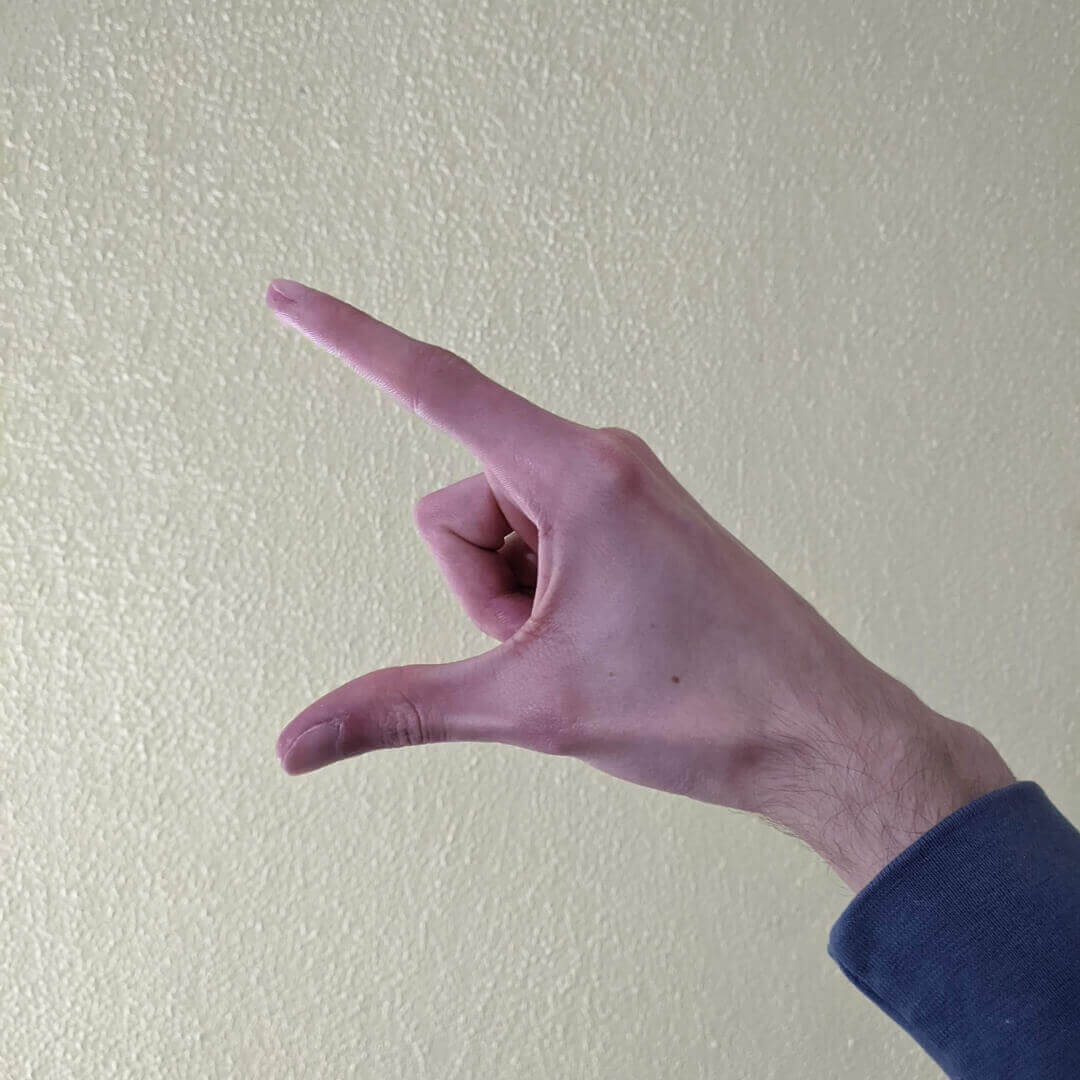
\includegraphics[width=0.25\textwidth]{introduccion/hand_open.jpg}}
    \subfloat{
\includegraphics[width=0.25\textwidth]{introduccion/hand_closed.jpg}}
    \subfloat{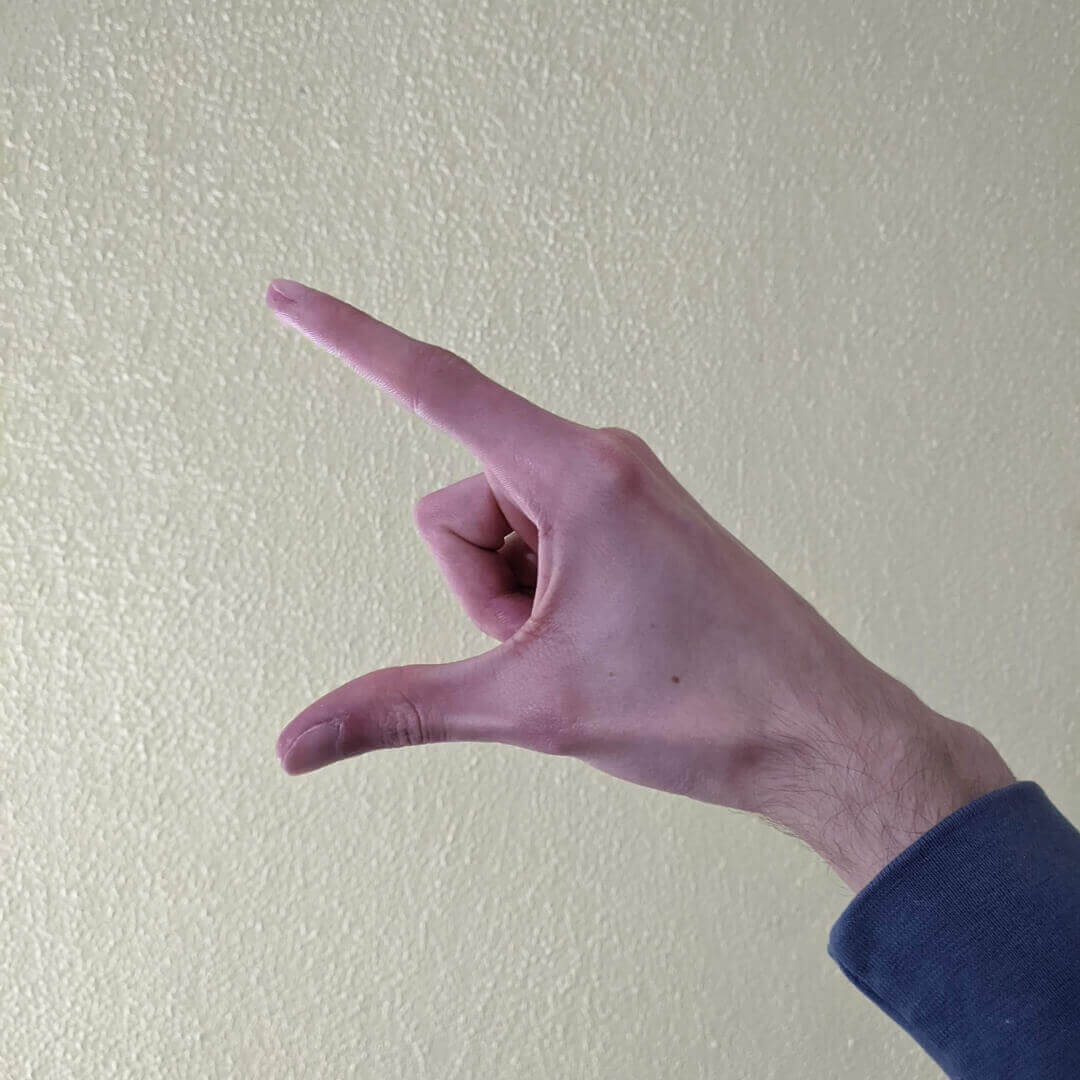
\includegraphics[width=0.25\textwidth]{introduccion/hand_open.jpg}}
    \subfloat{
\includegraphics[width=0.25\textwidth]{introduccion/hand_closed.jpg}}
    \caption{Finger-tapping test}
    \label{fig:finger-tapping-test}
\end{figure}

En los últimos años, la inteligencia artificial se ha convertido en una
herramienta de gran utilidad para el diagnóstico y tratamiento de enfermedades,
incluida la enfermedad de Parkinson. En este proyecto, se ha desarrollado un
sistema basado en inteligencia artificial para crear modelos de aprendizaje
automático capaces de detectar bradicinesia en un vídeo de un individuo
realizando el movimiento de <<finger-tapping>>.

Interactuar con los modelos creados de forma directa puede resultar complicado
si no se dispone de ciertos conocimientos previos sobre programación e
inteligencia artificial. Con el objetivo de facilitar esta tarea para un usuario
estándar se ha desarrollado una aplicación web que simplifica el uso de los
modelos.

Los resultados obtenidos indican que los modelos creados son capaces de detectar
la enfermedad de Parkinson con bastante precisión, lo que sugiere que podrían
ser de utilidad para la realización de un diagnóstico inicial, pero nunca
sustituyente de una evaluación médica, sobre el estado de la enfermedad. Además,
el enfoque basado en vídeo es fácil de usar y no es invasivo, lo que lo hace
potencialmente útil en entornos clínicos y de telemedicina.

Por último, me gustaría dar las gracias a todos aquellos que han dedicado su
tiempo y esfuerzo a la obtención de los vídeos utilizados para entrenar los
modelos, incluyendo la Asociación de Parkinson de Burgos, el personal del
Hospital Universitario de Burgos y el equipo de la Dra. Esther Cubo.
